\documentclass[aspectratio=169]{beamer}
\usetheme{metropolis}           % Use metropolis theme
\metroset{numbering=fraction}
\usepackage{tikz}
\usetikzlibrary{positioning}
\usetikzlibrary{arrows,backgrounds,automata,decorations.shapes,decorations.pathmorphing,decorations.markings,decorations.text,positioning,shapes.geometric}

\tikzstyle{place}=[circle,draw=blue!50,fill=blue!20,thick, inner sep=0pt,minimum size=6mm]
\tikzstyle{transition}=[rectangle,draw=black!50,fill=black!20,thick, inner sep=0pt,minimum size=4mm]

\tikzstyle{block}=[rectangle,draw=black, thick, inner sep=5pt]
\tikzstyle{bullet}=[circle,draw=black, fill=black, thin, inner sep=2pt]

\tikzstyle{pre}=[<-,shorten <=1pt,>=stealth',semithick]
\tikzstyle{post}=[->,shorten >=1pt,>=stealth',semithick]
\tikzstyle{bi}=[<->,shorten >=1pt,shorten <=1pt, >=stealth',semithick]

\tikzstyle{mut}=[-,>=stealth',semithick]

\tikzstyle{treereset}=[dashed,->, shorten >=1pt,>=stealth',thin]

\pgfdeclarelayer{edgelayer}
\pgfdeclarelayer{nodelayer}
\pgfsetlayers{edgelayer,nodelayer,main}

\tikzstyle{none}=[inner sep=0pt]
\tikzstyle{rn}=[circle,fill=Red,draw=Black,line width=0.8 pt]
\tikzstyle{gn}=[circle,fill=Lime,draw=Black,line width=0.8 pt]
\tikzstyle{yn}=[circle,fill=Yellow,draw=Black,line width=0.8 pt]
\tikzstyle{empty}=[circle,fill=White,draw=Black]
\tikzstyle{bw} = [rectangle, draw, fill=blue!20, 
    text width=4em, text centered, rounded corners, minimum height=2em]

\usepackage{float}
\usepackage{makecell}
\usepackage{fancyvrb}
\usepackage{listings}
\usepackage[export]{adjustbox}
\usepackage{caption}
\usepackage{alltt}
\title{Lecture 7 \\ Android Graphics and Intents}
\date{May 24, 2016}
\author{Patrick Lam \\ Jeff Zarnett \\ Michael Giannikouris}
\institute{Department of Electrical and Computer Engineering}
\setbeamertemplate{caption}{\raggedright\insertcaption\par}
\setbeamersize{text margin left=12pt,text margin right=12pt}
\newcommand{\putat}[3]{\begin{picture}(0,0)(0,0)\put(#1,#2){#3}\end{picture}} % just a shorthand

\newenvironment{deflist}
{ \begin{description}
    \setlength{\itemsep}{6pt}
    \setlength{\parskip}{0pt}
    \setlength{\parsep}{0pt}     }
{ \end{description}              } 

\newenvironment{splitslide}
{
\centering
\begin{tabular}{@{}p{0.50\textwidth} | p{0.025\textwidth}@{} p{0.4\textwidth}@{}}
}
{
\end{tabular}
}

\newcounter{tmpnumSlide}
\newcounter{tmpnumNote}

 \newcommand\mnote[1]{%
   \addtocounter{tmpnumSlide}{1}
   \ifdefined\showcues {~\tiny\fbox{\arabic{tmpnumSlide}}}\fi
   \note{\setlength{\parskip}{1ex}\addtocounter{tmpnumNote}{1}\textbf{\Large \arabic{tmpnumNote}:} {#1\par}}}


\begin{document}
\maketitle

\section*{Graphics in Android}



%%%%%%%%%%%%%%%%%%%%%%%%%%%%%%%%%%%%%%%%%%%%%%%%%%%%%%%%%%%%%%%%%%%%%%%%%%%%%%%%%%%%
% XML versus Programmatic Construction
%%%%%%%%%%%%%%%%%%%%%%%%%%%%%%%%%%%%%%%%%%%%%%%%%%%%%%%%%%%%%%%%%%%%%%%%%%%%%%%%%%%%
\begin{frame}{XML versus Programmatic Construction}
Use the right tool for the job! \\
\vspace{1em}
XML = more safety:
\begin{itemize}
\item Select and place items ahead of time.
\item Don't need the emulator to see how things will look.
\item More error checking.
\end{itemize}
~\\
Java Code = more flexibility:
\begin{itemize}
\item Can choose widgets based on user input or computations.
\item Can use loops, etc to generate related items.
\item Less error checking.
\end{itemize}
\end{frame}
%%%%%%%%%%%%%%%%%%%%%%%%%%%%%%%%%%%%%%%%%%%%%%%%%%%%%%%%%%%%%%%%%%%%%%%%%%%%%%%%%%%%




%%%%%%%%%%%%%%%%%%%%%%%%%%%%%%%%%%%%%%%%%%%%%%%%%%%%%%%%%%%%%%%%%%%%%%%%%%%%%%%%%%%%
% Putting Graphics on the Screen
%%%%%%%%%%%%%%%%%%%%%%%%%%%%%%%%%%%%%%%%%%%%%%%%%%%%%%%%%%%%%%%%%%%%%%%%%%%%%%%%%%%%
\begin{frame}[fragile]{Putting Graphics on the Screen}
\Large
Two choices:
\begin{itemize}
\item use a {\tt View} (easier; infrequent updates); or
\item paint to a {\tt Canvas} (more complicated, many updates).
\end{itemize}
\vspace{1em}
Let's look at some \texttt{View}s.
\end{frame}
%%%%%%%%%%%%%%%%%%%%%%%%%%%%%%%%%%%%%%%%%%%%%%%%%%%%%%%%%%%%%%%%%%%%%%%%%%%%%%%%%%%%



%%%%%%%%%%%%%%%%%%%%%%%%%%%%%%%%%%%%%%%%%%%%%%%%%%%%%%%%%%%%%%%%%%%%%%%%%%%%%%%%%%%%
% Main class: {\tt Drawable}
%%%%%%%%%%%%%%%%%%%%%%%%%%%%%%%%%%%%%%%%%%%%%%%%%%%%%%%%%%%%%%%%%%%%%%%%%%%%%%%%%%%%
\begin{frame}[fragile]{Main class: {\tt Drawable}}
\Large
Represents ``something that can be drawn'', e.g.
\begin{itemize}
\item BitmapDrawable
\item ShapeDrawable
\item PictureDrawable
\item etc.
\end{itemize}
\end{frame}
%%%%%%%%%%%%%%%%%%%%%%%%%%%%%%%%%%%%%%%%%%%%%%%%%%%%%%%%%%%%%%%%%%%%%%%%%%%%%%%%%%%%



%%%%%%%%%%%%%%%%%%%%%%%%%%%%%%%%%%%%%%%%%%%%%%%%%%%%%%%%%%%%%%%%%%%%%%%%%%%%%%%%%%%%
% Drawing to a View
%%%%%%%%%%%%%%%%%%%%%%%%%%%%%%%%%%%%%%%%%%%%%%%%%%%%%%%%%%%%%%%%%%%%%%%%%%%%%%%%%%%%
\begin{frame}[fragile]{Drawing to a View}
\Large
As always with Android, either:
\begin{itemize}
\item through XML, or
\item programmatically
\end{itemize}
\end{frame}
%%%%%%%%%%%%%%%%%%%%%%%%%%%%%%%%%%%%%%%%%%%%%%%%%%%%%%%%%%%%%%%%%%%%%%%%%%%%%%%%%%%%



%%%%%%%%%%%%%%%%%%%%%%%%%%%%%%%%%%%%%%%%%%%%%%%%%%%%%%%%%%%%%%%%%%%%%%%%%%%%%%%%%%%%
% Bitmaps through ImageView
%%%%%%%%%%%%%%%%%%%%%%%%%%%%%%%%%%%%%%%%%%%%%%%%%%%%%%%%%%%%%%%%%%%%%%%%%%%%%%%%%%%%
\begin{frame}[fragile]{Bitmaps through ImageView}
Easiest way\footnote{\tiny Thanks to: \url{http://www.cs.umd.edu/class/fall2010/CMSC498G/CMSC498G/Slides_files/Graphics.pptx}}:  
\begin{itemize}
\item put a picture ({\tt PNG}, {\tt JPG} or {\tt GIF}) in {\tt res/drawables}.
\item use an {\tt ImageView} to include it on the screen.
\end{itemize}
{\scriptsize
\begin{verbatim}
  // Instantiate an ImageView and define its properties programmatically
  ImageView i = new ImageView(this);
  i.setImageResource(R.drawable.my_image);
  // set the ImageView bounds to match the Drawable's dimensions
  i.setAdjustViewBounds(true);
  i.setLayoutParams(new Gallery.LayoutParams
      (LayoutParams.WRAP_CONTENT, LayoutParams.WRAP_CONTENT));
  // Add the ImageView to the layout and 
  //  set the layout as the content view
  mLinearLayout.addView(i);
\end{verbatim}
}
\vspace{-0.5em}
\tiny from: \url{http://developer.android.com/guide/topics/graphics/2d-graphics.html}
\vspace{1em}
\end{frame}
%%%%%%%%%%%%%%%%%%%%%%%%%%%%%%%%%%%%%%%%%%%%%%%%%%%%%%%%%%%%%%%%%%%%%%%%%%%%%%%%%%%%



%%%%%%%%%%%%%%%%%%%%%%%%%%%%%%%%%%%%%%%%%%%%%%%%%%%%%%%%%%%%%%%%%%%%%%%%%%%%%%%%%%%%
% Bitmaps through ImageView XML
%%%%%%%%%%%%%%%%%%%%%%%%%%%%%%%%%%%%%%%%%%%%%%%%%%%%%%%%%%%%%%%%%%%%%%%%%%%%%%%%%%%%
\begin{frame}[fragile]{Bitmaps through ImageView XML}
Again, you need the appropriate drawable in the {\tt res/drawables} directory.\\[1em]
Note: harder to go wrong here.

\begin{verbatim}
  <ImageView
    android:id="@+id/imageView1"
    android:layout_height="wrap_content"
    android:layout_width="wrap_content"
    android:src="@drawable/myImage" />
\end{verbatim}
\end{frame}
%%%%%%%%%%%%%%%%%%%%%%%%%%%%%%%%%%%%%%%%%%%%%%%%%%%%%%%%%%%%%%%%%%%%%%%%%%%%%%%%%%%%



%%%%%%%%%%%%%%%%%%%%%%%%%%%%%%%%%%%%%%%%%%%%%%%%%%%%%%%%%%%%%%%%%%%%%%%%%%%%%%%%%%%%
% Bitmaps through ImageView XML
%%%%%%%%%%%%%%%%%%%%%%%%%%%%%%%%%%%%%%%%%%%%%%%%%%%%%%%%%%%%%%%%%%%%%%%%%%%%%%%%%%%%
\begin{frame}[fragile]{Drawing on a ShapeDrawable}
\Large
Primitive shapes: 
\begin{itemize}
\item PathShape---lines;
\item RectShape---rectangles;
\item OvalShape---ovals and rings;
\end{itemize}
\vspace{2em}
Once again, we put these into an {\tt ImageView}.
\end{frame}
%%%%%%%%%%%%%%%%%%%%%%%%%%%%%%%%%%%%%%%%%%%%%%%%%%%%%%%%%%%%%%%%%%%%%%%%%%%%%%%%%%%%



%%%%%%%%%%%%%%%%%%%%%%%%%%%%%%%%%%%%%%%%%%%%%%%%%%%%%%%%%%%%%%%%%%%%%%%%%%%%%%%%%%%%
% Bitmaps through ImageView XML
%%%%%%%%%%%%%%%%%%%%%%%%%%%%%%%%%%%%%%%%%%%%%%%%%%%%%%%%%%%%%%%%%%%%%%%%%%%%%%%%%%%%
\begin{frame}[fragile]{Shapes from XML}
Again, you need the appropriate drawable in the {\tt res/drawables} directory.\\[1em]

In the Layout XML:
\begin{verbatim}
  <ImageView android:id="@+id/imageView2"
    android:src="@drawable/cyan_shape" ... />
\end{verbatim}

Next, we create an XML for the drawable itself:
\begin{verbatim}
  <shape android:shape="oval" ... >
    <size android:width="160px" 
          android:height="160px" />
    <solid android:color="#7f00ffff" />
  </shape>
\end{verbatim}
\end{frame}
%%%%%%%%%%%%%%%%%%%%%%%%%%%%%%%%%%%%%%%%%%%%%%%%%%%%%%%%%%%%%%%%%%%%%%%%%%%%%%%%%%%%



%%%%%%%%%%%%%%%%%%%%%%%%%%%%%%%%%%%%%%%%%%%%%%%%%%%%%%%%%%%%%%%%%%%%%%%%%%%%%%%%%%%%
% Bitmaps through ImageView XML
%%%%%%%%%%%%%%%%%%%%%%%%%%%%%%%%%%%%%%%%%%%%%%%%%%%%%%%%%%%%%%%%%%%%%%%%%%%%%%%%%%%%
\begin{frame}[fragile]{Shapes, programmatically}
Everything you can do in XML, you can do in code.

{\small
\begin{verbatim}
  private class MyDrawableView extends ImageView {
    private ShapeDrawable mDrawable;
    public MyDrawableView(Context context, int color) {
      ...
      mDrawable = new ShapeDrawable(new OvalShape());
      mDrawable.getPaint().setColor(color);
      mDrawable.setBounds(0, 0, size, size);
      mDrawable.setAlpha(alpha);
    }
    protected void onDraw(Canvas canvas) {
      mDrawable.draw(canvas);
    }
  }
\end{verbatim}
}
\end{frame}
%%%%%%%%%%%%%%%%%%%%%%%%%%%%%%%%%%%%%%%%%%%%%%%%%%%%%%%%%%%%%%%%%%%%%%%%%%%%%%%%%%%%



%%%%%%%%%%%%%%%%%%%%%%%%%%%%%%%%%%%%%%%%%%%%%%%%%%%%%%%%%%%%%%%%%%%%%%%%%%%%%%%%%%%%
% Bitmaps through ImageView XML
%%%%%%%%%%%%%%%%%%%%%%%%%%%%%%%%%%%%%%%%%%%%%%%%%%%%%%%%%%%%%%%%%%%%%%%%%%%%%%%%%%%%
\begin{frame}[fragile]{Shapes, programmatically}
In the Activity's {\tt onCreate()}:
\begin{verbatim}
  MyDrawableView magentaView = 
    new MyDrawableView(this, Color.MAGENTA);
    
  magentaView.setLayoutParams
    (new LinearLayout.LayoutParams(160, 160));
    
  addView(magentaView);
\end{verbatim}
\end{frame}
%%%%%%%%%%%%%%%%%%%%%%%%%%%%%%%%%%%%%%%%%%%%%%%%%%%%%%%%%%%%%%%%%%%%%%%%%%%%%%%%%%%%



%%%%%%%%%%%%%%%%%%%%%%%%%%%%%%%%%%%%%%%%%%%%%%%%%%%%%%%%%%%%%%%%%%%%%%%%%%%%%%%%%%%%
% Bitmaps through ImageView XML
%%%%%%%%%%%%%%%%%%%%%%%%%%%%%%%%%%%%%%%%%%%%%%%%%%%%%%%%%%%%%%%%%%%%%%%%%%%%%%%%%%%%
\begin{frame}{9-patches}
\begin{columns}
\begin{column}{0.02\textwidth}\end{column}
\begin{column}{0.65\textwidth}
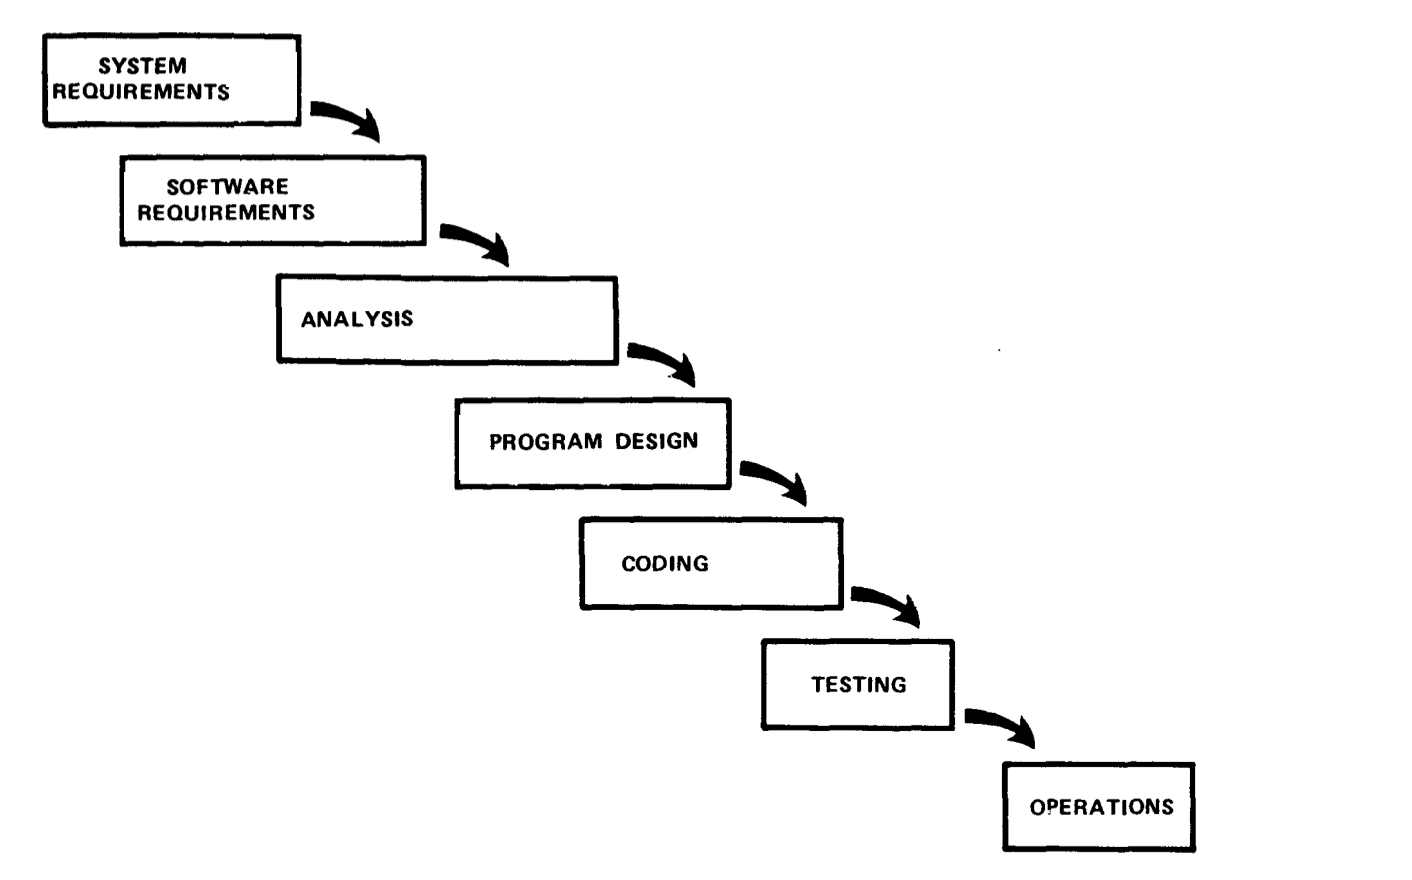
\includegraphics[width=0.95\textwidth]{img/concurrent-engineering.png}
\end{column}
\begin{column}{0.02\textwidth}\end{column}
\begin{column}{0.27\textwidth}
I manually stretched the boxes using a graphics editor.\\
\end{column}
\begin{column}{0.03\textwidth}\end{column}
\end{columns}
\end{frame}
%%%%%%%%%%%%%%%%%%%%%%%%%%%%%%%%%%%%%%%%%%%%%%%%%%%%%%%%%%%%%%%%%%%%%%%%%%%%%%%%%%%%



%%%%%%%%%%%%%%%%%%%%%%%%%%%%%%%%%%%%%%%%%%%%%%%%%%%%%%%%%%%%%%%%%%%%%%%%%%%%%%%%%%%%
% Bitmaps through ImageView XML
%%%%%%%%%%%%%%%%%%%%%%%%%%%%%%%%%%%%%%%%%%%%%%%%%%%%%%%%%%%%%%%%%%%%%%%%%%%%%%%%%%%%
\begin{frame}{9-patches: automatic stretching}
\vspace{1em}
\begin{columns}
\begin{column}{0.02\textwidth}\end{column}
\begin{column}{0.60\textwidth}
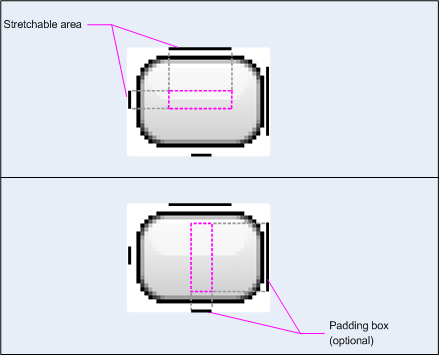
\includegraphics[height=0.90\textheight]{img/ninepatch_raw.png} \\
\end{column}
\begin{column}{0.02\textwidth}\end{column}
\begin{column}{0.33\textwidth}
\raggedright
\texttt{NinePatchDrawable} can stretch your images automatically! \\
\vspace{2em}
Just use a {\tt .9.png} file.  Edit using {\tt tools/draw9patch}. \\
\end{column}
\begin{column}{0.03\textwidth}\end{column}
\end{columns}
\end{frame}
%%%%%%%%%%%%%%%%%%%%%%%%%%%%%%%%%%%%%%%%%%%%%%%%%%%%%%%%%%%%%%%%%%%%%%%%%%%%%%%%%%%%



\section*{Android Intents}



%%%%%%%%%%%%%%%%%%%%%%%%%%%%%%%%%%%%%%%%%%%%%%%%%%%%%%%%%%%%%%%%%%%%%%%%%%%%%%%%%%%%
% Intents
%%%%%%%%%%%%%%%%%%%%%%%%%%%%%%%%%%%%%%%%%%%%%%%%%%%%%%%%%%%%%%%%%%%%%%%%%%%%%%%%%%%%
\begin{frame}{Intents}
\Large
So far we only examined an Activity in isolation. \\
\vspace{1em}
For the labs, you won't need anything more. \\
\vspace{1em}
In real apps, there's usually multiple activities. \\
\vspace{1em}
We link them with Intents.
\end{frame}
%%%%%%%%%%%%%%%%%%%%%%%%%%%%%%%%%%%%%%%%%%%%%%%%%%%%%%%%%%%%%%%%%%%%%%%%%%%%%%%%%%%%



%%%%%%%%%%%%%%%%%%%%%%%%%%%%%%%%%%%%%%%%%%%%%%%%%%%%%%%%%%%%%%%%%%%%%%%%%%%%%%%%%%%%
% Intents
%%%%%%%%%%%%%%%%%%%%%%%%%%%%%%%%%%%%%%%%%%%%%%%%%%%%%%%%%%%%%%%%%%%%%%%%%%%%%%%%%%%%
\begin{frame}{Intents}
\Large
An \emph{Intent} specifies a request or describes an event. \\
\vspace{1em}
Intents let you start another Activity and optionally provide data, or you can broadcast an event to the system. \\
\vspace{1em}
As usual we have a class for this called.....wait for it....\pause\texttt{Intent}.
\end{frame}
%%%%%%%%%%%%%%%%%%%%%%%%%%%%%%%%%%%%%%%%%%%%%%%%%%%%%%%%%%%%%%%%%%%%%%%%%%%%%%%%%%%%



%%%%%%%%%%%%%%%%%%%%%%%%%%%%%%%%%%%%%%%%%%%%%%%%%%%%%%%%%%%%%%%%%%%%%%%%%%%%%%%%%%%%
% Intents
%%%%%%%%%%%%%%%%%%%%%%%%%%%%%%%%%%%%%%%%%%%%%%%%%%%%%%%%%%%%%%%%%%%%%%%%%%%%%%%%%%%%
\begin{frame}[fragile]{Intents}
\Large
The simplest possible Intent explicitly names the Activity it would like to start. \\
\vspace{1em}
\large
\begin{Verbatim}
  Intent intent = new Intent(this, OtherActivity.class);
  startActivity(intent);
\end{Verbatim}
\end{frame}
%%%%%%%%%%%%%%%%%%%%%%%%%%%%%%%%%%%%%%%%%%%%%%%%%%%%%%%%%%%%%%%%%%%%%%%%%%%%%%%%%%%%



%%%%%%%%%%%%%%%%%%%%%%%%%%%%%%%%%%%%%%%%%%%%%%%%%%%%%%%%%%%%%%%%%%%%%%%%%%%%%%%%%%%%
% Intent: Request Example
%%%%%%%%%%%%%%%%%%%%%%%%%%%%%%%%%%%%%%%%%%%%%%%%%%%%%%%%%%%%%%%%%%%%%%%%%%%%%%%%%%%%
\begin{frame}{Intent: Request Example}
\Large
The Map activity puts up links to web pages 
\& phone numbers. \\
\vspace{1em}
Upon clicking one of these items, Map broadcasts either the \textbf{web browser}
Intent or the \textbf{call} Intent. \\
\vspace{1em}
The Map trusts that some other application will handle the Intent.
\end{frame}
%%%%%%%%%%%%%%%%%%%%%%%%%%%%%%%%%%%%%%%%%%%%%%%%%%%%%%%%%%%%%%%%%%%%%%%%%%%%%%%%%%%%



%%%%%%%%%%%%%%%%%%%%%%%%%%%%%%%%%%%%%%%%%%%%%%%%%%%%%%%%%%%%%%%%%%%%%%%%%%%%%%%%%%%%
% Intent: Event Example
%%%%%%%%%%%%%%%%%%%%%%%%%%%%%%%%%%%%%%%%%%%%%%%%%%%%%%%%%%%%%%%%%%%%%%%%%%%%%%%%%%%%
\begin{frame}{Intent: Event Example}
\Large
The system broadcasts an Intent when the phone
enters flight mode.
\end{frame}
%%%%%%%%%%%%%%%%%%%%%%%%%%%%%%%%%%%%%%%%%%%%%%%%%%%%%%%%%%%%%%%%%%%%%%%%%%%%%%%%%%%%



%%%%%%%%%%%%%%%%%%%%%%%%%%%%%%%%%%%%%%%%%%%%%%%%%%%%%%%%%%%%%%%%%%%%%%%%%%%%%%%%%%%%
% How Intents Work
%%%%%%%%%%%%%%%%%%%%%%%%%%%%%%%%%%%%%%%%%%%%%%%%%%%%%%%%%%%%%%%%%%%%%%%%%%%%%%%%%%%%
\begin{frame}{How Intents Work}
\Large
One component broadcasts an Intent. \\
\vspace{1em}
Then, 0 or more components receive the Intent. \\
\vspace{1em}
Android may pick a component to act upon the Intent.
\end{frame}
%%%%%%%%%%%%%%%%%%%%%%%%%%%%%%%%%%%%%%%%%%%%%%%%%%%%%%%%%%%%%%%%%%%%%%%%%%%%%%%%%%%%



%%%%%%%%%%%%%%%%%%%%%%%%%%%%%%%%%%%%%%%%%%%%%%%%%%%%%%%%%%%%%%%%%%%%%%%%%%%%%%%%%%%%
% Choosing the Handler
%%%%%%%%%%%%%%%%%%%%%%%%%%%%%%%%%%%%%%%%%%%%%%%%%%%%%%%%%%%%%%%%%%%%%%%%%%%%%%%%%%%%
\begin{frame}{Choosing the Handler}
\begin{center}
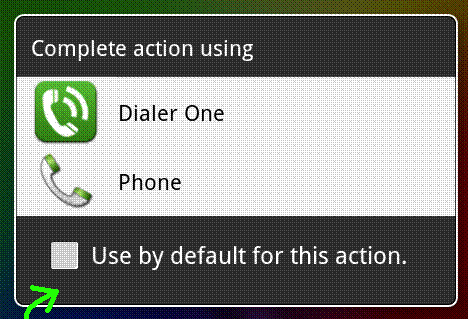
\includegraphics[height=.5\textheight]{img/completeaction.png}
\end{center}
\begin{tiny}(Image from stackoverflow.com)\end{tiny} \\
\vspace{0.5em}
In this case, the user is asked to choose.
\end{frame}
%%%%%%%%%%%%%%%%%%%%%%%%%%%%%%%%%%%%%%%%%%%%%%%%%%%%%%%%%%%%%%%%%%%%%%%%%%%%%%%%%%%%



%%%%%%%%%%%%%%%%%%%%%%%%%%%%%%%%%%%%%%%%%%%%%%%%%%%%%%%%%%%%%%%%%%%%%%%%%%%%%%%%%%%%
% An Intent in Action
%%%%%%%%%%%%%%%%%%%%%%%%%%%%%%%%%%%%%%%%%%%%%%%%%%%%%%%%%%%%%%%%%%%%%%%%%%%%%%%%%%%%
\begin{frame}{An Intent in Action}
\centering
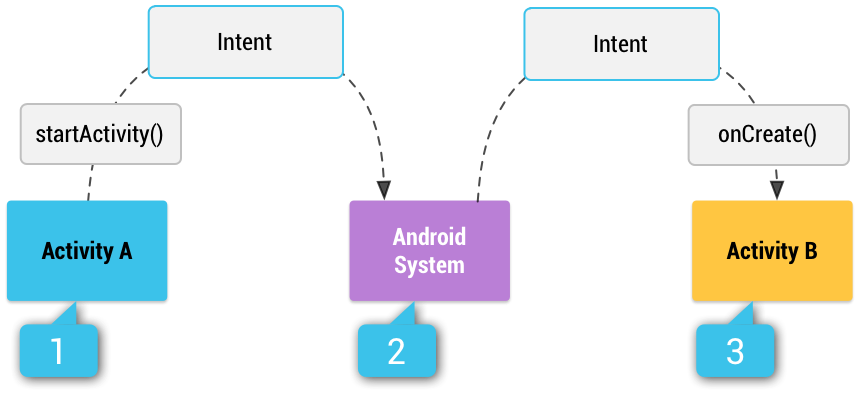
\includegraphics[height=0.8\textheight]{img/intent-filters@2x.png} \\
\begin{tiny}https://developer.android.com/guide/components/intents-filters.html\end{tiny}
\end{frame}
%%%%%%%%%%%%%%%%%%%%%%%%%%%%%%%%%%%%%%%%%%%%%%%%%%%%%%%%%%%%%%%%%%%%%%%%%%%%%%%%%%%%



\section*{Parts of an Intent}



%%%%%%%%%%%%%%%%%%%%%%%%%%%%%%%%%%%%%%%%%%%%%%%%%%%%%%%%%%%%%%%%%%%%%%%%%%%%%%%%%%%%
% Parts of an Intent
%%%%%%%%%%%%%%%%%%%%%%%%%%%%%%%%%%%%%%%%%%%%%%%%%%%%%%%%%%%%%%%%%%%%%%%%%%%%%%%%%%%%
\begin{frame}{Parts of an Intent}
\Large
Each intent contains an \emph{action} which represents the requested
action, along with optional \emph{data}. Some common Android actions: \\
\vspace{2em}
\hspace*{2em} \begin{tabular}{ll}
ACTION\_MAIN & Launch an activity \\
ACTION\_DIAL & Dial a phone number \\
ACTION\_SEARCH & Perform a search
\end{tabular}
\end{frame}
%%%%%%%%%%%%%%%%%%%%%%%%%%%%%%%%%%%%%%%%%%%%%%%%%%%%%%%%%%%%%%%%%%%%%%%%%%%%%%%%%%%%



%%%%%%%%%%%%%%%%%%%%%%%%%%%%%%%%%%%%%%%%%%%%%%%%%%%%%%%%%%%%%%%%%%%%%%%%%%%%%%%%%%%%
% Parts of an Intent
%%%%%%%%%%%%%%%%%%%%%%%%%%%%%%%%%%%%%%%%%%%%%%%%%%%%%%%%%%%%%%%%%%%%%%%%%%%%%%%%%%%%
\begin{frame}[fragile]{Parts of an Intent}
\large
These two code fragments yield identical Intents with an action (but no data): \\
\normalsize
\begin{Verbatim}
new Intent(Intent.ACTION_EDIT);
\end{Verbatim}
OR \\
\begin{Verbatim}
Intent intent = new Intent();
intent.setAction(Intent.ACTION_EDIT);
\end{Verbatim}
\end{frame}
%%%%%%%%%%%%%%%%%%%%%%%%%%%%%%%%%%%%%%%%%%%%%%%%%%%%%%%%%%%%%%%%%%%%%%%%%%%%%%%%%%%%



%%%%%%%%%%%%%%%%%%%%%%%%%%%%%%%%%%%%%%%%%%%%%%%%%%%%%%%%%%%%%%%%%%%%%%%%%%%%%%%%%%%%
% Parts of an Intent
%%%%%%%%%%%%%%%%%%%%%%%%%%%%%%%%%%%%%%%%%%%%%%%%%%%%%%%%%%%%%%%%%%%%%%%%%%%%%%%%%%%%
\begin{frame}{Parts of an Intent}
\large
The \emph{data} is the payload of the event. \\
\vspace{1em}
Android intent data is in
URI (Universal Resource Identifier) format\footnote{What's a URI? It's
like a URL. The exact distinction is unimportant for ECE155.}.  \\
\vspace{1em}
The obvious thing to put into data is a web address, but a URI can contain many other data formats. \\
\vspace{1em}
For example, a telephone number URI: \texttt{tel:+1-800-555-5555}.
\end{frame}
%%%%%%%%%%%%%%%%%%%%%%%%%%%%%%%%%%%%%%%%%%%%%%%%%%%%%%%%%%%%%%%%%%%%%%%%%%%%%%%%%%%%



%%%%%%%%%%%%%%%%%%%%%%%%%%%%%%%%%%%%%%%%%%%%%%%%%%%%%%%%%%%%%%%%%%%%%%%%%%%%%%%%%%%%
% Parts of an Intent
%%%%%%%%%%%%%%%%%%%%%%%%%%%%%%%%%%%%%%%%%%%%%%%%%%%%%%%%%%%%%%%%%%%%%%%%%%%%%%%%%%%%
\begin{frame}[fragile]{Parts of an Intent}
\large
Intents.....now with data!\\
\vspace{1em}
Notice that \texttt{Intent} takes a \texttt{Uri} object as data, which we create from a String. \\
\vspace{2em}
\begin{Verbatim}[fontsize=\normalsize]
new Intent(Intent.ACTION_DIAL, Uri.parse("tel:6175551212"));
\end{Verbatim}
OR \\
\begin{Verbatim}
Intent intent = new Intent(Intent.ACTION_DIAL);
intent.setData(Uri.parse("tel:6175551212"));
\end{Verbatim}
\end{frame}
%%%%%%%%%%%%%%%%%%%%%%%%%%%%%%%%%%%%%%%%%%%%%%%%%%%%%%%%%%%%%%%%%%%%%%%%%%%%%%%%%%%%



%%%%%%%%%%%%%%%%%%%%%%%%%%%%%%%%%%%%%%%%%%%%%%%%%%%%%%%%%%%%%%%%%%%%%%%%%%%%%%%%%%%%
% Parts of an Intent
%%%%%%%%%%%%%%%%%%%%%%%%%%%%%%%%%%%%%%%%%%%%%%%%%%%%%%%%%%%%%%%%%%%%%%%%%%%%%%%%%%%%
\begin{frame}{Parts of an Intent}
\Large
You can also tell Android what type of data to expect. \\
\vspace{1em}
Use the {\tt setType} method. Example: {\tt
  intent.setType("audio/mp3");} \\
\vspace{1em}
This is optional. 
\end{frame}
%%%%%%%%%%%%%%%%%%%%%%%%%%%%%%%%%%%%%%%%%%%%%%%%%%%%%%%%%%%%%%%%%%%%%%%%%%%%%%%%%%%%



%%%%%%%%%%%%%%%%%%%%%%%%%%%%%%%%%%%%%%%%%%%%%%%%%%%%%%%%%%%%%%%%%%%%%%%%%%%%%%%%%%%%
% Intent Extras
%%%%%%%%%%%%%%%%%%%%%%%%%%%%%%%%%%%%%%%%%%%%%%%%%%%%%%%%%%%%%%%%%%%%%%%%%%%%%%%%%%%%
\begin{frame}{Intent Extras}
\Large
Beyond the data, Intents may also contain \emph{extras}.  \\
\vspace{1em}
Extras consist of key-value pairs.  \\
\vspace{1em}
They contain more information than what can easily be put in a URI.
\end{frame}
%%%%%%%%%%%%%%%%%%%%%%%%%%%%%%%%%%%%%%%%%%%%%%%%%%%%%%%%%%%%%%%%%%%%%%%%%%%%%%%%%%%%



%%%%%%%%%%%%%%%%%%%%%%%%%%%%%%%%%%%%%%%%%%%%%%%%%%%%%%%%%%%%%%%%%%%%%%%%%%%%%%%%%%%%
% Intent Extras Example
%%%%%%%%%%%%%%%%%%%%%%%%%%%%%%%%%%%%%%%%%%%%%%%%%%%%%%%%%%%%%%%%%%%%%%%%%%%%%%%%%%%%
\begin{frame}[fragile]{Intent Extras Example}
\begin{Verbatim}[fontsize=\large]
Intent intent = new Intent(Intent.ACTION_SEND);
intent.putExtra(android.content.Intent.EXTRA_EMAIL,
  new String[] {
    "p.lam@ece.uwaterloo.ca", "root@uwaterloo.ca"
  });
\end{Verbatim}
\vspace{1em}
\end{frame}
%%%%%%%%%%%%%%%%%%%%%%%%%%%%%%%%%%%%%%%%%%%%%%%%%%%%%%%%%%%%%%%%%%%%%%%%%%%%%%%%%%%%



%%%%%%%%%%%%%%%%%%%%%%%%%%%%%%%%%%%%%%%%%%%%%%%%%%%%%%%%%%%%%%%%%%%%%%%%%%%%%%%%%%%%
% Intent Flags
%%%%%%%%%%%%%%%%%%%%%%%%%%%%%%%%%%%%%%%%%%%%%%%%%%%%%%%%%%%%%%%%%%%%%%%%%%%%%%%%%%%%
\begin{frame}{Intent Flags}
\large
Finally, Intents may also contain \emph{flags}. \\
\vspace{1em}
These modify how the
Intent gets launched and how it will be processed by the recipient. \\
\vspace{1em}
They don't affect which activity gets launched. \\
\vspace{1em}
Examples: {\tt FLAG\_ACTIVITY\_NO\_HISTORY} and 
{\tt FLAG\_ACTIVITY\_RESET\_TASK\_IF\_NEEDED}.
\end{frame}
%%%%%%%%%%%%%%%%%%%%%%%%%%%%%%%%%%%%%%%%%%%%%%%%%%%%%%%%%%%%%%%%%%%%%%%%%%%%%%%%%%%%



%%%%%%%%%%%%%%%%%%%%%%%%%%%%%%%%%%%%%%%%%%%%%%%%%%%%%%%%%%%%%%%%%%%%%%%%%%%%%%%%%%%%
% For Your Reference
%%%%%%%%%%%%%%%%%%%%%%%%%%%%%%%%%%%%%%%%%%%%%%%%%%%%%%%%%%%%%%%%%%%%%%%%%%%%%%%%%%%%
\begin{frame}{For Your Reference}
\Large
Android has standards for various Actions, Extras, and Flags, and that's where we're getting all the names you saw in this section. \\
\vspace{2em}
\url{https://developer.android.com/reference/android/content/Intent.html}
\end{frame}
%%%%%%%%%%%%%%%%%%%%%%%%%%%%%%%%%%%%%%%%%%%%%%%%%%%%%%%%%%%%%%%%%%%%%%%%%%%%%%%%%%%%



\section*{Intent Resolution}



%%%%%%%%%%%%%%%%%%%%%%%%%%%%%%%%%%%%%%%%%%%%%%%%%%%%%%%%%%%%%%%%%%%%%%%%%%%%%%%%%%%%
% Intent Resolution
%%%%%%%%%%%%%%%%%%%%%%%%%%%%%%%%%%%%%%%%%%%%%%%%%%%%%%%%%%%%%%%%%%%%%%%%%%%%%%%%%%%%
\begin{frame}{Intent Resolution}
\large
We've seen that we can explicitly name the Activity we want to launch. \\
\vspace{1em}
We've seen that we can implicitly launch an activity by describing what we want. \\
\vspace{1em}
In either case, we use {\tt startActivity} to launch the intent.\\
\vspace{1em}
\textbf{Implicit intent resolution:} system searches the
available Activities, using the Intent's action, data
and category.
\end{frame}
%%%%%%%%%%%%%%%%%%%%%%%%%%%%%%%%%%%%%%%%%%%%%%%%%%%%%%%%%%%%%%%%%%%%%%%%%%%%%%%%%%%%



%%%%%%%%%%%%%%%%%%%%%%%%%%%%%%%%%%%%%%%%%%%%%%%%%%%%%%%%%%%%%%%%%%%%%%%%%%%%%%%%%%%%
% Responding to Intent Resolution Requests
%%%%%%%%%%%%%%%%%%%%%%%%%%%%%%%%%%%%%%%%%%%%%%%%%%%%%%%%%%%%%%%%%%%%%%%%%%%%%%%%%%%%
\begin{frame}[fragile]{Responding to Intent Resolution Requests}
In your application's manifest, there's an XML tag for each activity.
That tag can take an \emph{intent filter} describing the Intents
that the activity is prepared to handle. For example: \\
\vspace{0.5em}
{\scriptsize 
\begin{verbatim}
<activity
    android:name=".BrowserActivity"
    android:label="@string/app_name" >
    <intent-filter>
        <action android:name="android.intent.action.VIEW" />

        <category android:name="android.intent.category.DEFAULT" />

        <data android:scheme="http" />
    </intent-filter>
</activity>
\end{verbatim}
}
\vspace{0.5em}
This activity is able to view any URI that begins with {\tt http}.
\end{frame}
%%%%%%%%%%%%%%%%%%%%%%%%%%%%%%%%%%%%%%%%%%%%%%%%%%%%%%%%%%%%%%%%%%%%%%%%%%%%%%%%%%%%



\section*{Receiving Results from an Activity}



%%%%%%%%%%%%%%%%%%%%%%%%%%%%%%%%%%%%%%%%%%%%%%%%%%%%%%%%%%%%%%%%%%%%%%%%%%%%%%%%%%%%
% Receiving Activity Results
%%%%%%%%%%%%%%%%%%%%%%%%%%%%%%%%%%%%%%%%%%%%%%%%%%%%%%%%%%%%%%%%%%%%%%%%%%%%%%%%%%%%
\begin{frame}[fragile]{Receiving Activity Results}
When you launch a sub-activity via an Intent, sometimes you're hoping for a result
back from that activity. \\
\vspace{0.5em}
For instance, you may be asking for the
user to pick a contact from the contact list. \\
\vspace{0.5em}
Or you may be asking the
user for a favourite colour. \\
\vspace{0.5em}
The sub-activity should
create a new Intent and call its {\tt setResult} method: \\
\vspace{0.5em}
\begin{Verbatim}[fontsize=\normalsize]
  Intent retval = new Intent();
  retval.putExtra("color", "blue");
  setResult(RESULT_OK, retval);
\end{Verbatim}
\end{frame}
%%%%%%%%%%%%%%%%%%%%%%%%%%%%%%%%%%%%%%%%%%%%%%%%%%%%%%%%%%%%%%%%%%%%%%%%%%%%%%%%%%%%



%%%%%%%%%%%%%%%%%%%%%%%%%%%%%%%%%%%%%%%%%%%%%%%%%%%%%%%%%%%%%%%%%%%%%%%%%%%%%%%%%%%%
% Receiving Activity Results
%%%%%%%%%%%%%%%%%%%%%%%%%%%%%%%%%%%%%%%%%%%%%%%%%%%%%%%%%%%%%%%%%%%%%%%%%%%%%%%%%%%%
\begin{frame}[fragile]{Receiving Activity Results}
Then in the caller, we provide a new callback, {\tt onActivityResult()}. \\
\vspace{1em}
\begin{Verbatim}
  @Override
  protected void onActivityResult(int requestCode, 
                                  int resultCode, 
                                  Intent data) {
    if(resultCode == RESULT_OK && 
        requestCode == YOUR_REQUEST_CODE) {
      if(data.hasExtra("color")) {
        String myColour = data.getExtras().getString("color");
      }
    }
  }
\end{Verbatim}
\end{frame}
%%%%%%%%%%%%%%%%%%%%%%%%%%%%%%%%%%%%%%%%%%%%%%%%%%%%%%%%%%%%%%%%%%%%%%%%%%%%%%%%%%%%



%%%%%%%%%%%%%%%%%%%%%%%%%%%%%%%%%%%%%%%%%%%%%%%%%%%%%%%%%%%%%%%%%%%%%%%%%%%%%%%%%%%%
% Receiving Activity Results
%%%%%%%%%%%%%%%%%%%%%%%%%%%%%%%%%%%%%%%%%%%%%%%%%%%%%%%%%%%%%%%%%%%%%%%%%%%%%%%%%%%%
\begin{frame}[fragile]{Receiving Activity Results}
\Large
The {\tt requestCode} is an {\tt int} you provided when starting the
sub-activity for a result. \\
\vspace{1em}
\begin{Verbatim}
int REQUEST_CODE = 1;
startActivityForResult(intent, REQUEST_CODE);
\end{Verbatim}
\vspace{1em}
It allows you to distinguish different sub-activities you may have started.
\end{frame}
%%%%%%%%%%%%%%%%%%%%%%%%%%%%%%%%%%%%%%%%%%%%%%%%%%%%%%%%%%%%%%%%%%%%%%%%%%%%%%%%%%%%



%%%%%%%%%%%%%%%%%%%%%%%%%%%%%%%%%%%%%%%%%%%%%%%%%%%%%%%%%%%%%%%%%%%%%%%%%%%%%%%%%%%%
% Parts of an Intent
%%%%%%%%%%%%%%%%%%%%%%%%%%%%%%%%%%%%%%%%%%%%%%%%%%%%%%%%%%%%%%%%%%%%%%%%%%%%%%%%%%%%
\begin{frame}{Passing Data Using Intents}
Video: \\
\url{https://www.youtube.com/watch?v=0ism1OM0an0}
\end{frame}
%%%%%%%%%%%%%%%%%%%%%%%%%%%%%%%%%%%%%%%%%%%%%%%%%%%%%%%%%%%%%%%%%%%%%%%%%%%%%%%%%%%%


\section*{On Problem Solving}

\begin{frame}{The Key to Programming}
\large
The key to programming is simple. \\
\vspace{1em}
\begin{enumerate}
\item Determine where we are (point A).
\item Determine where we're trying to go (point B).
\item Find a series of steps to get us from A to B.
\end{enumerate}
\end{frame}


\begin{frame}{Math Problem Example}
\large
Suppose you haven't memorized the answer to $12 \times 13$.  \\
\vspace{1em}
Other than whipping out the calculator, what can you do? \\
\vspace{1em}
Break it down into a series of problems you know how to solve. \\
\vspace{0.25em}
$(12 x 10) + (12 x 3)$ \\
\vspace{1em}
We now have three problems, but they're small and easy. \\
\end{frame}




\begin{frame}{Decomposition}
Note: we have to know the rules of math to understand how the problem can be decomposed. \\
\vspace{1em}
In programming, the step you come up with might be a little bit too complicated for a computer or person to execute. \\
\vspace{1em}
So you break the items of step 3 down by repeating this process. \\
\vspace{1em}
Keep breaking it down until the steps are small enough for the computer to execute.
\end{frame}

\begin{frame}{Decomposition: Step Size}
\large
How small those steps are is a matter of what language and tools you are using. \\
\vspace{1em}
Imagine a Fourier Transform of a signal (fancy math).  \\
\vspace{1em}
If you're using an advanced language you might just write \texttt{FourierTransform(signal)}. \\
\vspace{1em}
Or you might have to write the transform at a low level.
\end{frame}

\begin{frame}{Key Lesson}
\Large
Decomposing the problem is the key.\\
\vspace{1em}
Learning the syntax of the language is another matter...
\end{frame}


\end{document}